\documentclass[a4 paper]{article}
% Set target color model to RGB
\usepackage[inner=2.0cm,outer=2.0cm,top=2.5cm,bottom=2.5cm]{geometry}
\usepackage{setspace}
\usepackage[rgb]{xcolor}
\usepackage{verbatim}
\usepackage{subcaption}
\usepackage{amsgen,amsmath,amstext,amsbsy,amsopn,tikz,amssymb}
\usepackage{fancyhdr}
\usepackage[colorlinks=true, urlcolor=blue,  linkcolor=blue, citecolor=blue]{hyperref}
\usepackage[colorinlistoftodos]{todonotes}
\usepackage{rotating}
\usepackage{enumitem}
\usepackage{float}
%\usetikzlibrary{through,backgrounds}
\hypersetup{%
pdfauthor={Aishik Mandal},%
pdftitle={Homework 1},%
pdfkeywords={Tikz,latex,bootstrap,uncertaintes},%
pdfcreator={PDFLaTeX},%
pdfproducer={PDFLaTeX},%
}
%\usetikzlibrary{shadows}
% \usepackage[francais]{babel}
\usepackage{booktabs}
% \input{macros.tex}

\newcommand{\ra}[1]{\renewcommand{\arraystretch}{#1}}

\newtheorem{thm}{Theorem}[section]
\newtheorem{prop}[thm]{Proposition}
\newtheorem{lem}[thm]{Lemma}
\newtheorem{cor}[thm]{Corollary}
\newtheorem{defn}[thm]{Definition}
\newtheorem{rem}[thm]{Remark}
\numberwithin{equation}{section}

\newcommand{\homework}[5]{
   \pagestyle{myheadings}
   \thispagestyle{plain}
   \newpage
   \setcounter{page}{1}
   \noindent
   \begin{center}
   \framebox{
      \vbox{\vspace{2mm}
    \hbox to 6.28in { {\bf Ethics for NLP: SS 2024 \hfill {\small (#2)}} }
       \vspace{6mm}
       \hbox to 6.28in { {\Large \hfill #1  \hfill} }
       \vspace{6mm}
       \hbox to 6.28in {  {\it Name: {\rm #3}
        %NetID: {\rm #4} 
        \hfill Matriculation No.: {\rm #5}} }
      \vspace{2mm}}
   }
   \end{center}
   \markboth{#5 -- #1}{#5 -- #1}
   \vspace*{4mm}
}

\newcommand{\problem}[2]{~\\\fbox{\textbf{Problem #1}}\newline\newline}
\newcommand{\subproblem}[1]{~\newline\textbf{(#1)}}
\newcommand{\D}{\mathcal{D}}
\newcommand{\Hy}{\mathcal{H}}
\newcommand{\VS}{\textrm{VS}}

\newcommand{\bbF}{\mathbb{F}}
\newcommand{\bbX}{\mathbb{X}}
\newcommand{\bI}{\mathbf{I}}
\newcommand{\bX}{\mathbf{X}}
\newcommand{\bY}{\mathbf{Y}}
\newcommand{\bepsilon}{\boldsymbol{\epsilon}}
\newcommand{\balpha}{\boldsymbol{\alpha}}
\newcommand{\bbeta}{\boldsymbol{\beta}}
\newcommand{\0}{\mathbf{0}}
\newcommand{\code}[1]{\texttt{#1}}


\begin{document}
\homework{Homework 1}{Due: 29 May 2024, 11:59pm}{Julian Steiner}{}{2669944}

%Read all the instructions carefully before you start working on the assignment, and before you make a submission.

\problem{2}{}

\subproblem{2.1}

% Comment on the bias you observed through this example

The results of this simple bias analysis show a clear difference in associations when "job" is paired with "men" vs. "woman". For "job" and "men", the associated words include other words like "managership", "managerial\_reigns", and "duties", which are could be linked to leadership or managerial roles. In contrary, "women" is associated words like "employment", "internships", "secretarial", "temping", which are stereotypically associated with gender-specific roles or entry-level positions and not with management positions. The reason could be a bias in the model, reflecting societal stereotypes where men are associated with higher-status positions and women with roles that are either remporary and lower-status.

% What kind of bias among label bias, selection bias, overamplification bias and semantic bias did you observe here?

\begin{itemize}
   \item Selection Bias: It could be possible, that the training corpus had overrepresented certain stereotypes or lacked diversity in depicting various roles across genders. This would lead to biased word associations.
   \item Semantic Bias: This type of bias can be observed as the meanings and associations of words learned by the model reflect societal stereotypes. The training data could contain biases in the meanings of words, leading the model to reinforce these biases in its predictions and associations.
   \item Overamplification Bias: The model might amplify existing societal biases more than they appear in the real world, leading to stronger biased associations.
\end{itemize}

\problem{2}

\subproblem{2.2.2}

Figure \ref{fig:prob_dist_valence_label_joy} show the probability distribution of predicting valence label of 1 for male and female with the emotion "joy". The female distribution has a slightly higher density in the most probability ranges, indicating that females might be more likely to be predicted as joyous compared to males.

\begin{figure}[H]
   \centering
   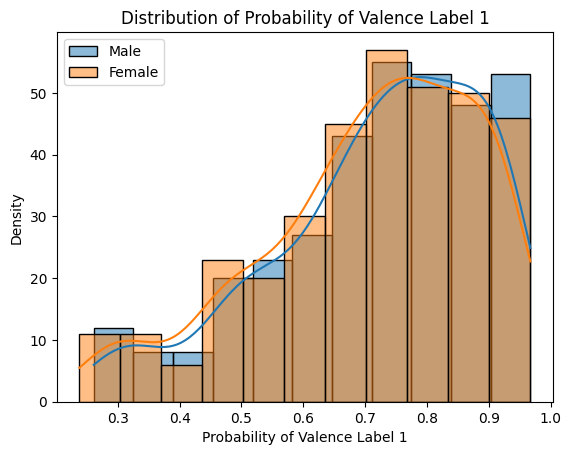
\includegraphics[width=0.5\linewidth]{Probability_Dist_Valence_Label_1_Joy}
   \caption{Probabilty Distribution of predicting valence of label 1 for male and female with emotion joy.}
   \label{fig:prob_dist_valence_label_joy}
\end{figure}

\problem{3}

The kind of biased behavior we observe here is about the error disparity. The distribution of errors here are different between the African-American and white speakers. The Word Error Rate (WER) is consistently higher for African-American speakers compared to white speakers.

\hfill \break

The result for this could be of multiple bias sources:

\begin{itemize}
   \item Label Bias: The labels used for training could be biased, for example, due to the annotators of the data. If the majority of the annotators were white speakers, it could be possible that this had led to a bias in the training data.

   \item Selection Bias: It could be possible that the training data does not adequately represent the diversity of the population using the system. The dataset could contain significantly more audio samples from white speakers than from African-American speakers. The result would be that the model will be better at recognizing patterns it has seen more frequently.

   \item Overamplification Bias: It could be possible that there is a overamplification bias. The model could overamphasize linguistic features that are more prevalent in white speech.

   \item Semantic Bias: It could be possible that the training data may not include sufficient representation of the linguistic styles common among African-American speakers. The consequence is that the model could have biases in how the interpret and process language from different groups.

   \item Design Bias: I don't think that the system should only work for white speaker and not for African-American speaker. It should work for both groups. It could be possible that more resource of white speakers were available to train the models. The consequence we can see in the results. The system perform suboptimally for the African-American speaker.
\end{itemize}


\end{document}
